\documentclass{article}
\usepackage{amsmath}
\usepackage{amsthm}
\usepackage{amssymb}
\usepackage{algorithm}
\usepackage{graphicx}
\usepackage[noend]{algpseudocode}
\usepackage{url}

\newlength\tindent
\setlength{\tindent}{\parindent}
\setlength{\parindent}{0pt}
\renewcommand{\indent}{\hspace*{\tindent}}

\newtheorem{thm}{Theorem}
\newtheorem{cor}{Corollary}[thm]
\newtheorem{lemma}{Lemma}[thm]

\title{Knapsack Problem}
\author{Daniel Braithwaite}

\begin{document}
	\pagenumbering{gobble}
	\maketitle
	\newpage
  	\pagenumbering{arabic}
  	
	\section{Dynamic Knapsack 0-1}  
		\subsection{Algorithm}
		
		 	Given a list of items $item_1,......item_n$, say we have a table T that in position T[i][j] stores the best solution's for packing items $item_1,....item_i$ into a bag with capacity j. We can use the following recurrence
			
			\begin{align}
				max
				\begin{cases}
					T[i-1][j]\\
					T[i-1][j-items[i].weight] + items[i].value
				\end{cases}
			\end{align}				
		
			\begin{algorithm}
				\begin{algorithmic}[1]
					\Procedure{dnamicKnapsack01}{$capacity, items$}
						\State $T \gets int[items.length][capacity+1]$
						
						\For{$i = 0, i < items.length, i \gets i+1$}
							\For{$j = 0, j < capacity+1, j \gets j+1$}
								\State Fill out cell based on recurrence
							\EndFor
						\EndFor
						
						\State $solution \gets [0....0]$ (n zeros)						
						
						\State $i \gets items.length-1$
						\State $j \gets capacity-1$
						
						\While{$j > 0$} \Comment{while we have available capacity} 
							\State Use recurrence to figure out what action we took to get this value
							\If{We took item $i$ to get here}
								\State $j \gets items[i].weight$
								
								\State $solution[i] \gets 1$
							\EndIf
							
							\State $i \gets i - 1$
						\EndWhile
						
					\EndProcedure
				\end{algorithmic}
			\end{algorithm}
		\subsection{Proof}
			We want to work our way towards the recurrence we used in the dynamic programming algorithm. Say we have $n$ items we are trying to put into a bag of capacity $C$. Ether we put the $n^{th}$ item in the bag or we didn't. From this we get the following two sub problems.
			
			\begin{enumerate}
				\item \textbf{We took the $n^{th}$ item:} Here we are solving the sub problem where we have items $item_1,.....,item_{n-1}$ and bag with capacity $C - item_n.weight$.
				
				\item \textbf{Didn't take $n^{th}$ item:} Here the sub problem is the items $item_1,.....,item_{n-1}$ and bag with capacity $C$.
			\end{enumerate}
			
			This observation gives us our recurrence, now we need to show optimal sub structure for both of these cases
			
			\begin{enumerate}
				\item Say we took the $n^{th}$ item. Let $S$ be set of items taken giving the optimal solution for this problem. Assume for a contradiction that $S - \{item_n\}$ isn't the optimal solution for the problem $item_1,.....,item_{n-1}$ with a bag of capacity $C - item_n.weight$. Let $S^\prime$ be an optimal solution for this sub problem. But then we could take $S^\prime$ and add $n$ back in. This would give us a better solution than $S$ for the whole problem. A contradiction!
				
				\item Now say we didn't take the $n^{th}$ item. Let $S$ be the optimal selection of items. Assume for a contradiction that $S$ is not the optimal solution for the sub problem $item_1,.....,item_{n-1}$ with capacity $C$. But then we could take a better solution say $S^\prime$, not choose the $n^{th}$ item and have a solution better than $S$. A contradiction!
			\end{enumerate}								
		
		Now we see the Knapsack 0-1 problem as optimal substructure. Now we must prove the algorithm is correct. First we look at filling out the table.\newline
		
		Fill out the table must be correct as we just proved the problem had optimal substructure using that recurrence. The last thing to show is that recovering the solution from the table is always correct.\newline
		
		To start this we see that this also uses the recurrence we defined to determine what action was taken. If an item was taken then we mark it as taken in the solution. With ether action we move back in the table to where that solution came from until we have $j$ at 0 which means that we have no more available capacity.		
		
		\subsection{Complexity}		
			\subsubsection{Filling Out Table}
				The main part of the algorithm cost is here. The table is of size $weight * numItems$ and no matter the input data the whole table has to be filed out. The cost of using the recurrence is $O(1)$. Therefore the cost for filling out the table is
		
				\begin{align}
					\theta(nC)
				\end{align}
				
			\subsubsection{Finding Solution}
				The cost of this involves moving through the table and recovering the decisions at each point. Finding what decision was made is $O(1)$. At worst case you would be moving one square in the table at a time. Therefore finding the solution has cost
				
				\begin{align}
					O(n + C)
				\end{align}
				
			\subsubsection{Overall Cost}
				Combing the cost of the previous sections we see this algorithm has the following cost
				
				\begin{align}
					\theta(nC)
				\end{align}
		
		\subsection{Testing}
			I plotted the lines for the best, average and worst case data this algorithm could encounter. I defined the worst case data to be as follows.
			
			\begin{enumerate}
				\item \textbf{Best Case} is when reconstructing the solution we can just do it all in one step. So for this to happen we set all the item values and weights to be the same.
				
				\item \textbf{Worst Case} is when we take as many steps through the table as possible. To get this we set all the weights to be 1.
				
				\item \textbf{Average Case} is just randomly generated data
			\end{enumerate}
			
			\begin{figure}[h]
				\vspace{3mm}
				\begin{center}
					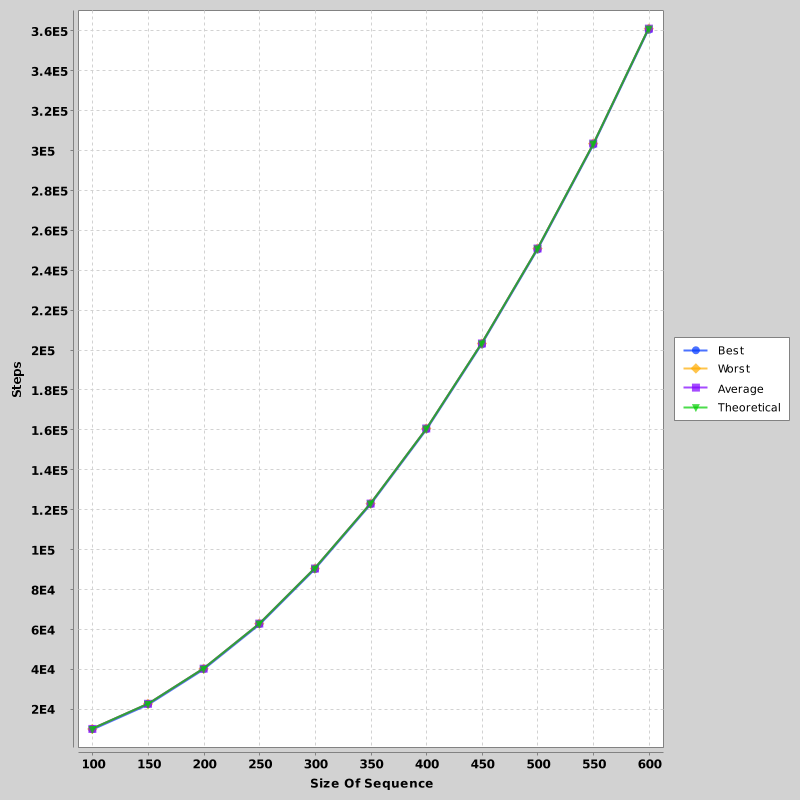
\includegraphics[scale=0.4]{Dynamic.png}
				\end{center}
			\end{figure}
			
			\break
			
			No matter the input for this algorithm the dynamic programming table will have to be filled. The only thing that will cause a difference will be how long it will take to recover the solution. However this cost is minimal compared to the cost of computing the table. So for some input size $n$ if we have best, worst or average case data the number of steps will be almost identical for all of them. This is why you can only see one line, as they are all overlapping. All the lines fit perfect with the theoretical.
		
			\break			
		
	\section{Brute Force Knapsack 0-N}
		\subsection{Algorithm}
			\begin{algorithm}
				\begin{algorithmic}[1]
					\Procedure{bruteforceKnapsack01}{$capacity, items$}
						\State $w, b \gets [0,.....,0]$ \Comment{number of entries equals items.length}

						\While{true}
							\State $w[0] \gets w[0] + 1$
							
							\For{index i in w} \Comment{Handle when we are taking to much of an item}
								\If{$w[i] > item_i.mutiplicity$}
									\State $w[i] \gets 0$
									\State $w[i+1] \gets w[i+1] + 1$
								\EndIf
							\EndFor
							
							\If{we have taken all of the last item} \Comment{this is true if we have enumerated all possible solutions}
								\State break
							\EndIf
							
							\State $weight \gets$ weight of possible solution w
							
							\If{$weight \leqslant capacity$}
								\State Store solution in b if the value is better
							\EndIf
						\EndWhile
						
						\Return b
					\EndProcedure				
					
				\end{algorithmic}
			\end{algorithm}		
		\subsection{Proof}		
			The brute force algorithm works by enumerating all the possible options and storing the one with the best value if its weight is less or equal to the capacity
		\subsection{Complexity}
			This algorithm has to enumerate all the possible combinations of items. No matter what the input data is (best, worst, average case) it will still have to enumerate all the solutions as it has no way of being able to tell if it has found the best one except for checking the all the remaining ones. We get the complexity to be 
			
			\begin{align}
				\theta(2^n)
			\end{align}
			
		\subsection{Testing}
			There is no best, worst or average case, as discussed in \textbf{2.3}. As such we only graphed the average case and the theoretical line. When graphing this we only ran it on very small data sets as it is a very inefficient algorithm.
			
			\begin{figure}[h]
				\vspace{3mm}
				\begin{center}
					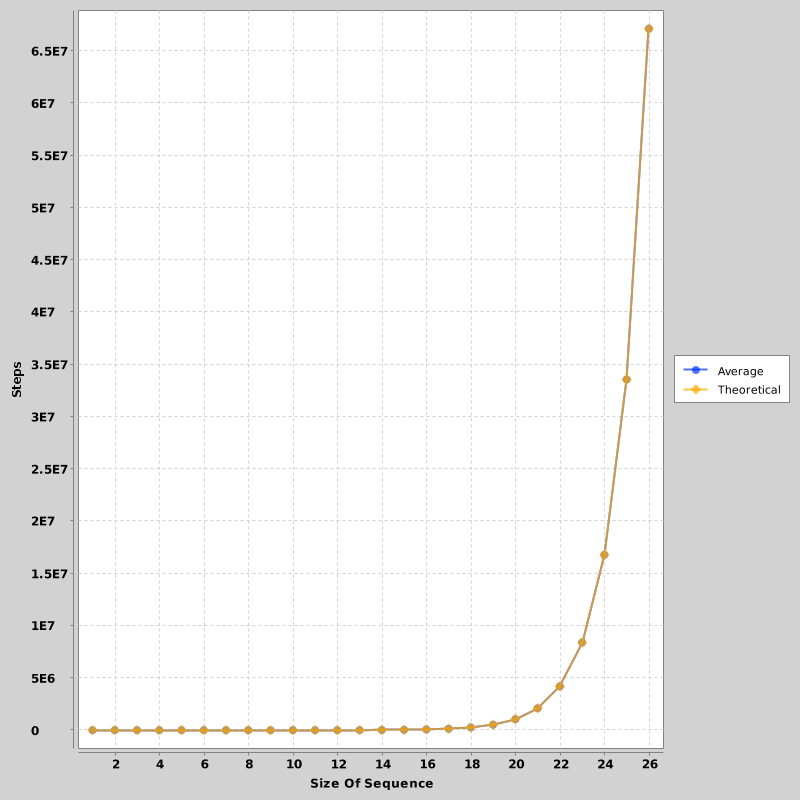
\includegraphics[scale=0.4]{BruteForce.png}
				\end{center}
			\end{figure}
			
			As you can see in the graph the average case line matches up perfectly with the theoretical line.
		
	\section{Problem Conversion 0-N to 0-1}
		The following 0-N algorithms will convert there 0-N knapsack problems to 0-1 problems. Here we will detail the algorithm for doing this with the cost. Rather than actually producing a new list of items and working with that we will create a mapping. Say our item list has size $n^\prime$ and this list represents $n$ items. Then our mapping take numbers in the range 0 to n and map them to numbers between 0 and $n^\prime$.
	
		\break	
				
		\subsection{Algorithm}
			\begin{algorithm}
				\begin{algorithmic}[1]
					\Procedure{createMapping}{$items$}
						\State $mapping \gets []$					
					
						\State $i \gets 0, j \gets 1, k \gets 0$
						\While{$k < items.length$}
							\State itemMapping.map(i to k)
							
							\If{$j = items[k].multiplicity$}
								\State $j \gets 0$
								\State $k \gets k + 1$
							\EndIf
							
							\State $i \gets i + 1$
							\State $j \gets j + 1$
						\EndWhile
						
						\Return mapping
					\EndProcedure
				\end{algorithmic}
			\end{algorithm}		
		\subsection{Proof}
			For each item passed in has a multiplicity (i.e. how many of that item we have) if we examine the algorithm we can clearly that it will create a mapping to an item item.multiplicity times. From this we see that the algorithm is correct.
			
		\subsection{Cost}
			We can clearly see that the loop is going to iterate exactly once for each of the $n$ items making the cost
			
			\begin{align}
				\theta(n)
			\end{align}				
		
		\break
		
	\section{Dynamic Knapsack 0-N}
		\subsection{Algorithm}
			Here we can use our previous 0-1 knapsack algorithm to solve this one. We just need to create an algorithm to convert a 0-N knapsack problem to a 0-1 problem and then once solved convert the solution back. The key difference being that if we want to access item k then really what we are doing is accessing the item k is mapped to ($mapping[k]$).
		
			\begin{algorithm}
				\begin{algorithmic}[1]
					\Procedure{dnamicKnapsack0N}{$capacity, items$}
						\State $mapping \gets createMapping(items)$	
						
						\State $T \gets int[mapping.length][capacity+1]$
						
						\For{$i = 0, i < mapping.length, i \gets i+1$}
							\For{$j = 0, j < capacity+1, j \gets j+1$}
								\State Fill out cell based on recurrence
							\EndFor
						\EndFor
						
						\State $solution \gets [0....0]$ \Comment{items.length number of 0's}						
						
						\State $i \gets items.length-1$
						\State $j \gets capacity-1$
						
						\While{$j > 0$} \Comment{while we have available capacity} 
							\State Use recurrence to figure out what action we took to get this value
							\If{We took item $i$ to get here}
								\State $j \gets items[mapping[i]].weight$
								
								\State $solution[mapping[i]]$++
							\EndIf
							
							\State $i \gets i - 1$
						\EndWhile
					\EndProcedure
				\end{algorithmic}
			\end{algorithm}
		\subsection{Proof}
			We see this algorithm works by converting the 0-N knapsack problem into a 0-1 knapsack problem and uses the 0-1 dynamic algorithm to solve it. The solution is then converted back to 0-N format.\newline
			
			We know that the conversion to 0-1 format is correct, we also know that the dynamic algorithm for solving the 0-1 knapsack is correct. So all we need prove is that the conversion of the solution back to 0-N is correct.\newline
			
			By inspecting the algorithm we see that our solution has an entry for each of the original items. We are using the recurrence to determine if an item was taken as we traverse the table. If an item was taken then we need to figure out what one of the original items it maps to and increment our count of that original item in the solution. We know we are able to do this correctly because our mapping is correct. 
		\subsection{Complexity}
		There are two parts for this algorithm we will explore the complexity for each of them and then we can come up with an overall complexity
			
		\subsubsection{Solving The 0-1 Problem}
			We already know the complexity of this and it is
		
			\begin{align}
				\theta(nC)
			\end{align}
		
		\subsubsection{Recovering Solution}
			The complexity of recovering the solution is the same as it was in the 0-1 dynamic solution. We only changed how the items where accessed
			
			\begin{align}
				\O(n + C)
			\end{align}
		
		\subsubsection{Overall Complexity}
			The dominating cost is still that  of solving the 0-1 Knapsack problem giving this algorithm
			
			\begin{align}
				\theta(nC)
			\end{align}
			
			\break
		\subsection{Testing}
			\textbf{Please Note:} For the testing of all the knapsack 0-N algorithms we used data where none of the items had a multiplicity over 1 (for simplicity). This \textbf{wouldn't} effect the results as the conversion will still run and the rest of the algorithm will run for the same amount of time had there been less input items but the same total n items\newline		
		
			We tested this data on the same type of best, average and worst case data as we did for the 0-1 dynamic knapsack and as expected got the same result. 
			
			\begin{figure}[h]
				\vspace{3mm}
				\begin{center}
					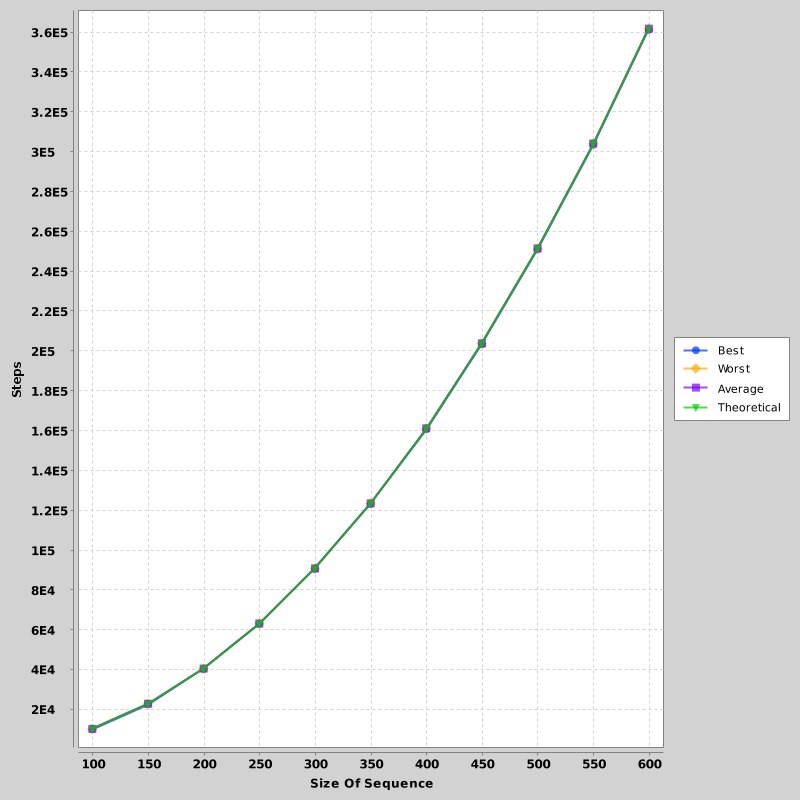
\includegraphics[scale=0.4]{Dynamic0N.png}
				\end{center}
			\end{figure}
			
			We can see that all the lines match up perfectly with the theoretical data
			
	
	\break			

	\section{Graph Search Knapsack 0-N}
		To start with we want to convert the 0-N problem to a 0-1 problem. This is so we can use a similar idea to the dynamic programming table\footnote{\url{http://courses.csail.mit.edu/6.006/fall11/rec/rec21_knapsack.pdf}}. Each node will be represented by the following triple $<i, j, value, previous>$ where $0 \leqslant i \leqslant numItems$ and $0 \leqslant j \leqslant capacity$ . The i and j mean the node contains the best solution for the items 0 to i-1 for a knapsack of capacity j.\newline\newline
		
		A node is connected to at most two others. Let $n$ be a node. The possibility's are ether we take item n.i or we don't. In the first case n is linked to a node where i = n.i + 1, and j = n.j + item[i] (as long as n.j + item[i] is $\leqslant$ capacity. In the second case n is linked to the node where i = n.i + 1, and j = n.j. As we are building the graph we want to keep track of the current best value of each node, along with that we keep track of the previous node that was used to get this value.
		
		For simplicity we will sometimes refer to a node as just <i,j>. Then we can refer to the value and previous node as <i,j>.value and <i,j>.previous
	
		\subsection{Algorithm}
			\begin{algorithm}
				\begin{algorithmic}[1]
					\Procedure{graphKnapsack0N}{$capacity, items$}
						\State $items^\prime \gets convertTo01Problem(items)$
						\State $fringe \gets []$
						\State add root node $<0, 0, 0, null>$
						
						\While{fringe is not empty}
							\State $current \gets node from fringe$
							\State remove current from fringe
						
							\If{$current.i + 1 > items^\prime$}
								\State return to top of loop
							\EndIf
							
							\State get node $<current.i + 1,current.j>$ if it doesn't exist add it to fringe.
							
							\State update $<current.i + 1,current.j>$ if our current path to the node is better
							
							\If{there is enough available weight to take item j}
								\State get node $<current.i + 1,current.j + items ^\prime[i].weight>$ if it doesn't exist add it to fringe
								\State update that node if there is a better path to it
							\EndIf
							
						\EndWhile
						
						\State $solution \gets [0,.....,0]$  \Comment{same length as items}
					\EndProcedure
				\end{algorithmic}
			\end{algorithm}
		
		\break
		\subsection{Proof}
			We will need to prove two things for this algorithm to be correct. First being that our method of generating the graph will explore all the possibility's. Second we need to show that we can recover the best path through the graph, thus giving us the optimal solution and finally show that the part of the algorithm that recovers the solution also correctly converts it back to a 0-N solution.	\newline	
		
			We think of nodes as representing a sub problem. For example the node $<2, 5>$ is saying we have considered the items 0 and 1, and that we have used up 5 of our total capacity. From here we have two choices ether we take item 2 (taking item 2 also depends on weather we have enough spare capacity) or we don't take item $i$. Meaning there is an edge between $<2, 5>$ and the nodes $<3, 5>$ and $<3, 5 + 1>$ (assuming the weight of item 2 is 1). If we make this more general and apply it to some node $<i, j>$ then clearly we are searching all the possible combinations. So if we store the node with the best value as we are building this binary tree then by the end we clearly will have a node that holds the best possible value\newline
			
			Now we have a node that can tell us the best value possible when trying to put all these items into a back with a known capacity. But what we are really interested in is the combination of items. As we are building the graph when we link two nodes with an edge, say  $n$ to $n^\prime$, we examine the current value of $n^\prime$ and see if the value of $n$ (plus the value of item $n.i$ we are taking it) is greater than it. If it is then we store $n$ as the previous node in $n^\prime$. We do this for all nodes so at the end we can just step back through the tree starting from the best node giving us the solution.\newline
			
			Finally we look at the part of the code that recovers the solution. This starts at the node in the graph that has the best value stepping back though the nodes using the previous value. At any iteration in the loop we have a node $n$ and the one before it $n_p$. We compare $n.j$ and $n_p.j$ if they are equal then we didn't take an item so just set $n$ to $n_p$. If they are not equal then we update the solution by using our mapping $solution[mapping[n_p.i]]$++. We increment the item $n_p.i$ as moving from $n_p$ to $n$ meant we where acting on the item $n_p.i$. This clearly gives us a 0-N solution that is correct.
			
		\subsection{Complexity}
			This algorithm has two components that we will explore separately.
			
			\subsubsection{Constructing The Graph}
				We can think of constructing the graph as traversing all the nodes in the graph. Which at worst case there will be as many nodes as there are cells in the dynamic programming table. However the key thing to note is that this is at worst, there often will be less nodes than this. Giving us the following complexity where n is the number of items (that is not the number of items in the input array but the sum of there multiplicity's) and C is the total capacity of the bag 
				
				\begin{align}
					O(nC)
				\end{align}										
				
			\subsubsection{Finding The Solution}
				At any node we know that it is connected to at most 2 nodes, there for what we generated is a binary tree. We also know the two following things. That there is going to be at most n + 1 layers (one for every possible value of i, $0 \leqslant i \leqslant n$). The second thing we know that as we are recovering the solution we are only stepping back through the tree. Therefore at worst we will have to step though the height of the tree giving us the complexity
				
				\begin{align}
					O(n+1)
				\end{align}
			
			\subsubsection{Overall Complexity}
				The dominating cost of the algorithm is that of constructing the graph so we get the algorithm complexity to be   
				
				\begin{align}
					O(nC)
				\end{align}	
				
		\subsection{Testing}
			The graph below displays the best, average and worst case for the graph search algorithm, we defined these as follows.
			
			\begin{enumerate}
				\item \textbf{Best Case} is when we can construct the graph with only having one layer. If we set all the items to have a capacity that will consume all available space we can get this.
				
				\item \textbf{Worst Case} is when we set each of the items to have a different weight, so for example for a set of 3 items we have $item_1.weight = 1, item_2.weight = 2,item_3.weight = 3$. This will give us the most possible nodes without much overlap. If we chose to do the same worst case data as we did for the dynamic programming we would do better than average as there would be a lot of overlap between nodes.
				
				\item \textbf{Average Case} is just randomly generated data
			\end{enumerate}
			
			\begin{figure}[h]
				\vspace{3mm}
				\begin{center}
					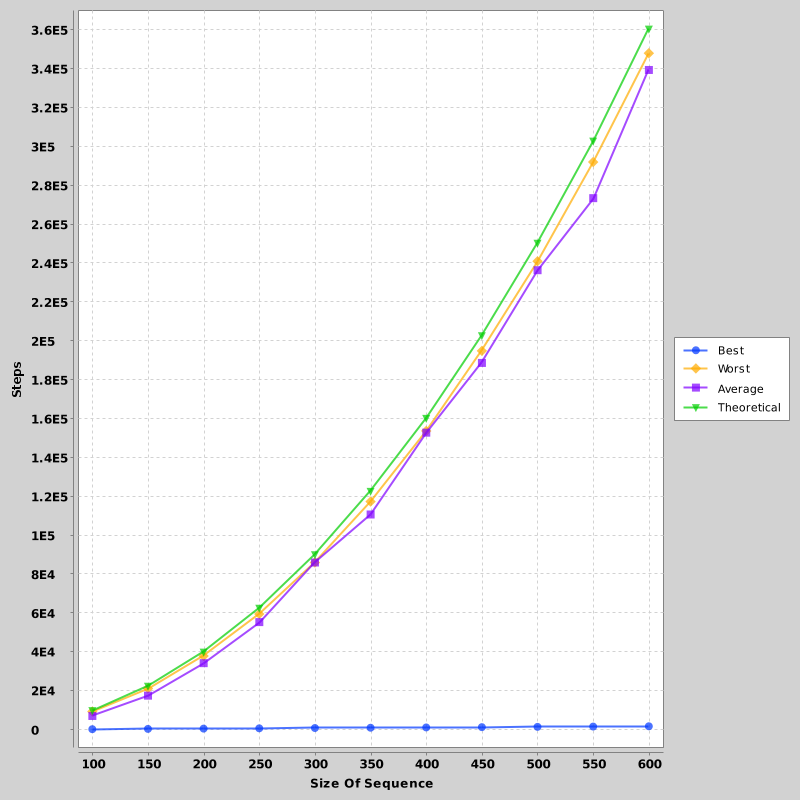
\includegraphics[scale=0.4]{Graph0N.png}
				\end{center}
			\end{figure}
					
			As we see in the graph this is much more varied than the other algorithms. The best case is very different from the average and worst case which are quite close together. However they are all less than the theoretical line which I graphed as $n*C + n + 1$ as this is the maximum number of steps the algorithm can take.		
			
			
	\section{Graph Search vs Dynamic}
		If we examine the order costs of the algorithm we would expect that the graph search would out perform the dynamic algorithm, or atleast perform the same as it. The graph search algorithm has a complexity of $O(nC)$ meaning it is bounded from above by $nC$. Compared to the complexity of the dynamic algorithm $\theta(nC)$ meaning it is bounded from above and below by $nC$.\newline

		If we examine the algorithms more closely we can also see this as noted in the dynamic algorithm complexity section the algorithm will always have to fill out the entire table no matter the input data. We also noted previously that in the graph search it was only worst case where we would have to traverse $nC$ number of nodes. \newline		
		
		We can conclude from this that the graph search algorithm will perform at most $nC$ steps where as the dynamic algorithm will always perform $nC$ steps.\newline
		
		We can also examine the cost of reconstructing the solution for each of the algorithms. Even here the graph search algorithm is faster, with a complexity of $O(n + 1)$ compared to the dynamic algorithm where recovering the solution is $O(n + C)$. \newline
		
		With this in mind we compare the best case of the dynamic algorithm and the worst case of the graph search.
		
		\begin{figure}[h]
			\vspace{3mm}
			\begin{center}
				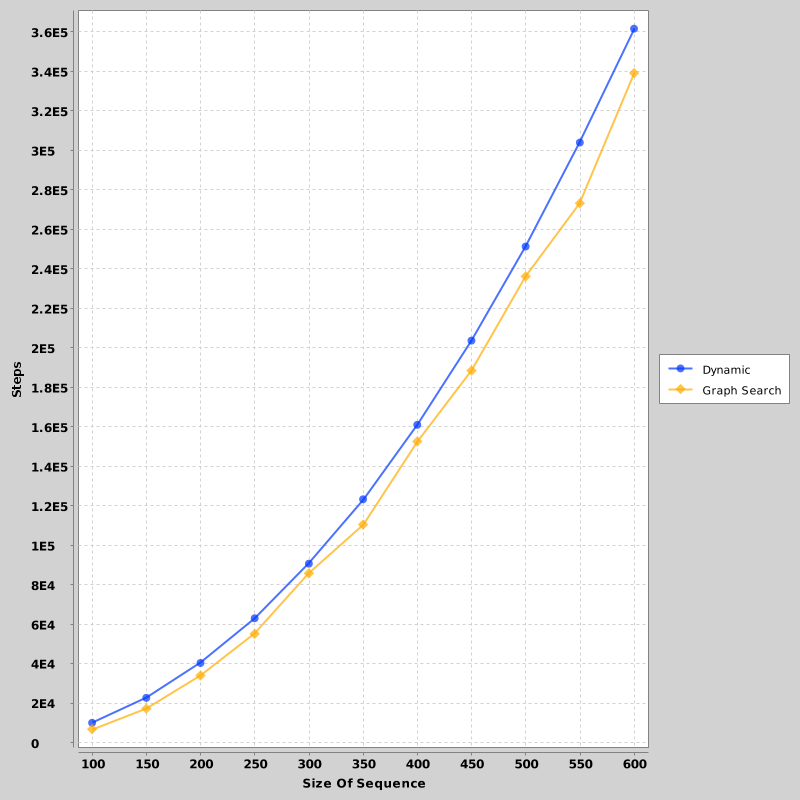
\includegraphics[scale=0.4]{DynamicGraphComparason.png}
			\end{center}
		\end{figure}
		
		As we can see in the graph the graph search algorithm clearly out performs the dynamic algorithm.
		
  			
\end{document}